% file: ThePhysicsOfInterstellar.tex
% AdS/CFT and Interstellar
% 
% github        : ernestyalumni
% linkedin      : ernestyalumni 
% wordpress.com : ernestyalumni
%
% This code is open-source, governed by the Creative Common license.  Use of this code is governed by the Caltech Honor Code: ``No member of the Caltech community shall take unfair advantage of any other member of the Caltech community.'' 
% 

\documentclass{beamer}
% cf. https://tex.stackexchange.com/questions/38352/resize-scale-equation-in-beamer
\usepackage{graphicx}% http;//ctan.org/pkg/graphicx

\usetheme{default}

% cf. https://tex.stackexchange.com/questions/79420/changing-font-style-using-beamer
\usefonttheme{structuresmallcapsserif} % using non standard fonts for beamer
\usefonttheme{serif} % default family is serif

\title{
	\centering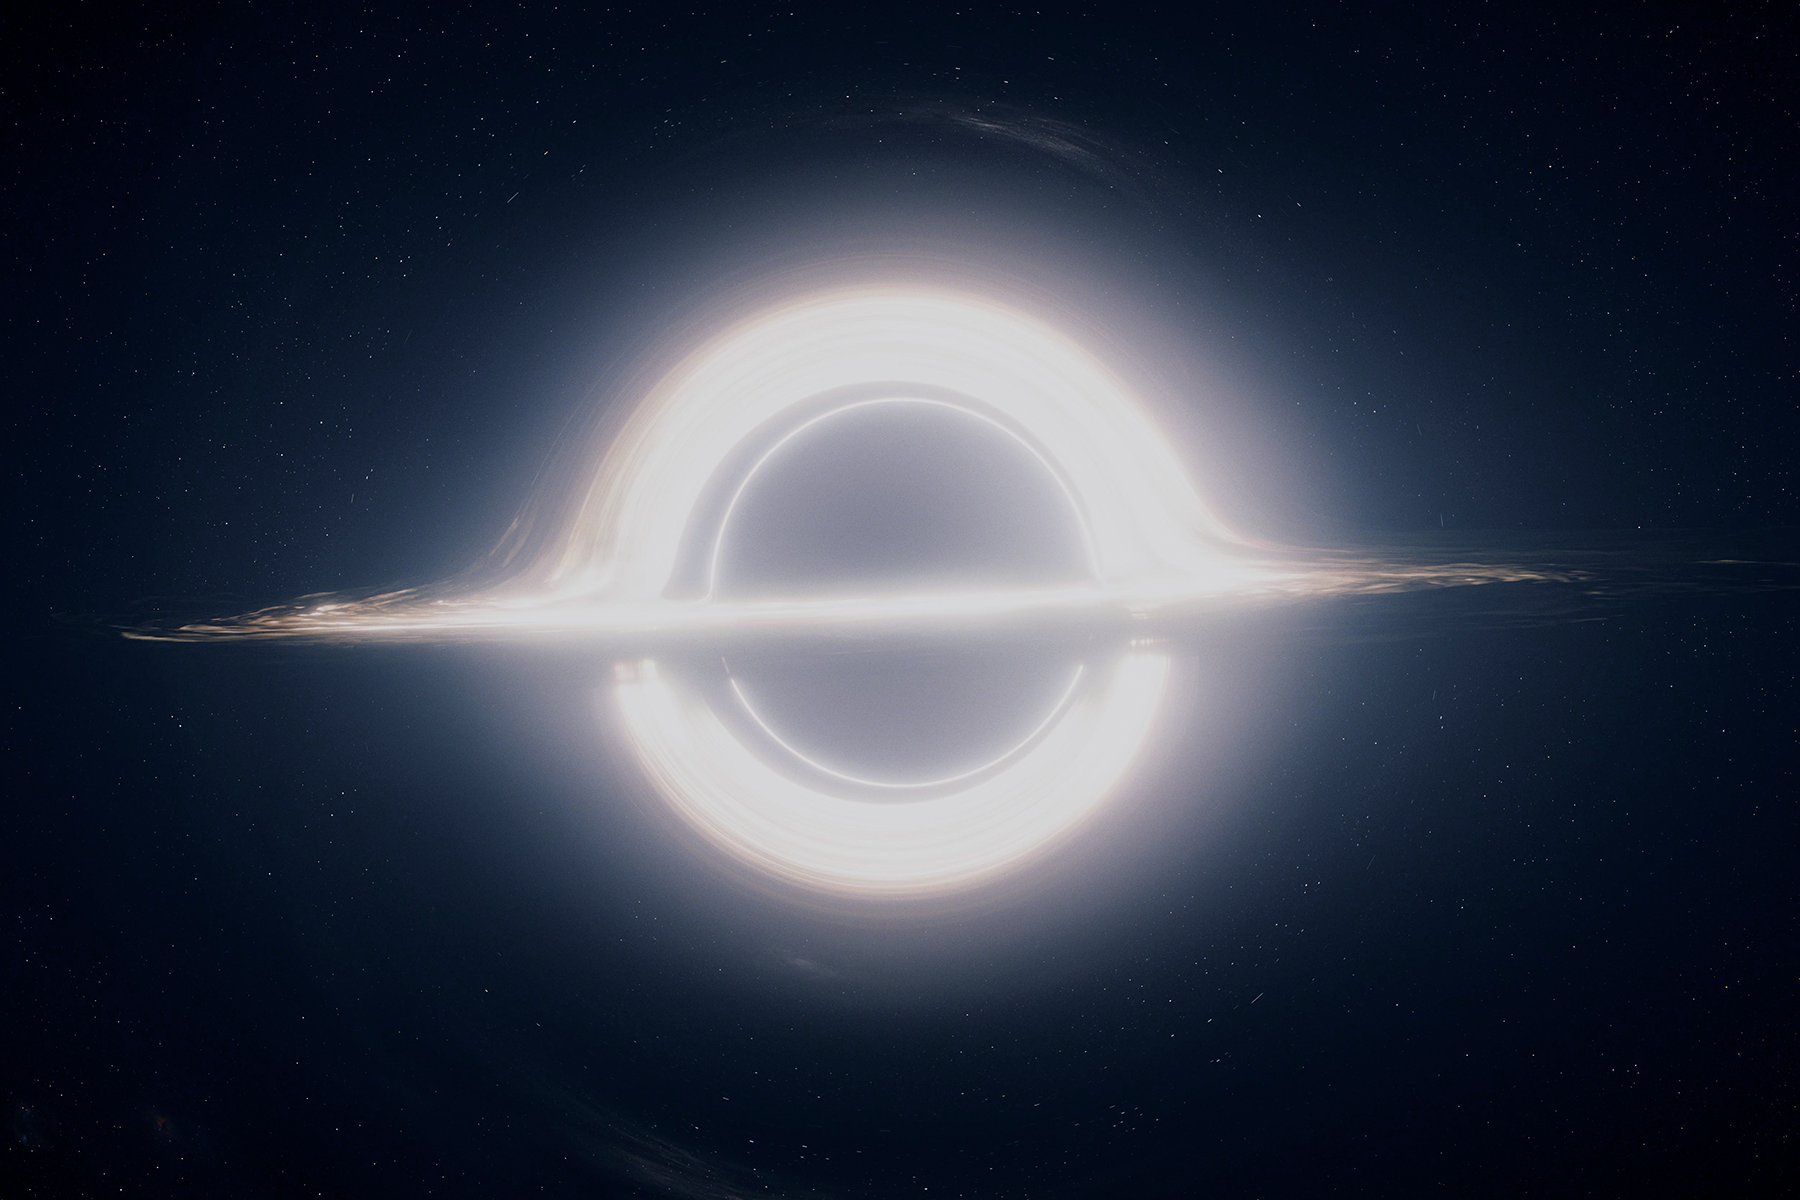
\includegraphics[width=0.85\textwidth]{images/ut_interstellarOpener_f.png}\\	
	The Physics of Interstellar
}
\author{Ernest Yeung}

\begin{document}
	% Title page frame.
	\begin{frame}
		\titlepage
	\end{frame}
	\begin{frame}{Gravitational lensing of spinning (Kerr) black holes}
		\begin{figure}
			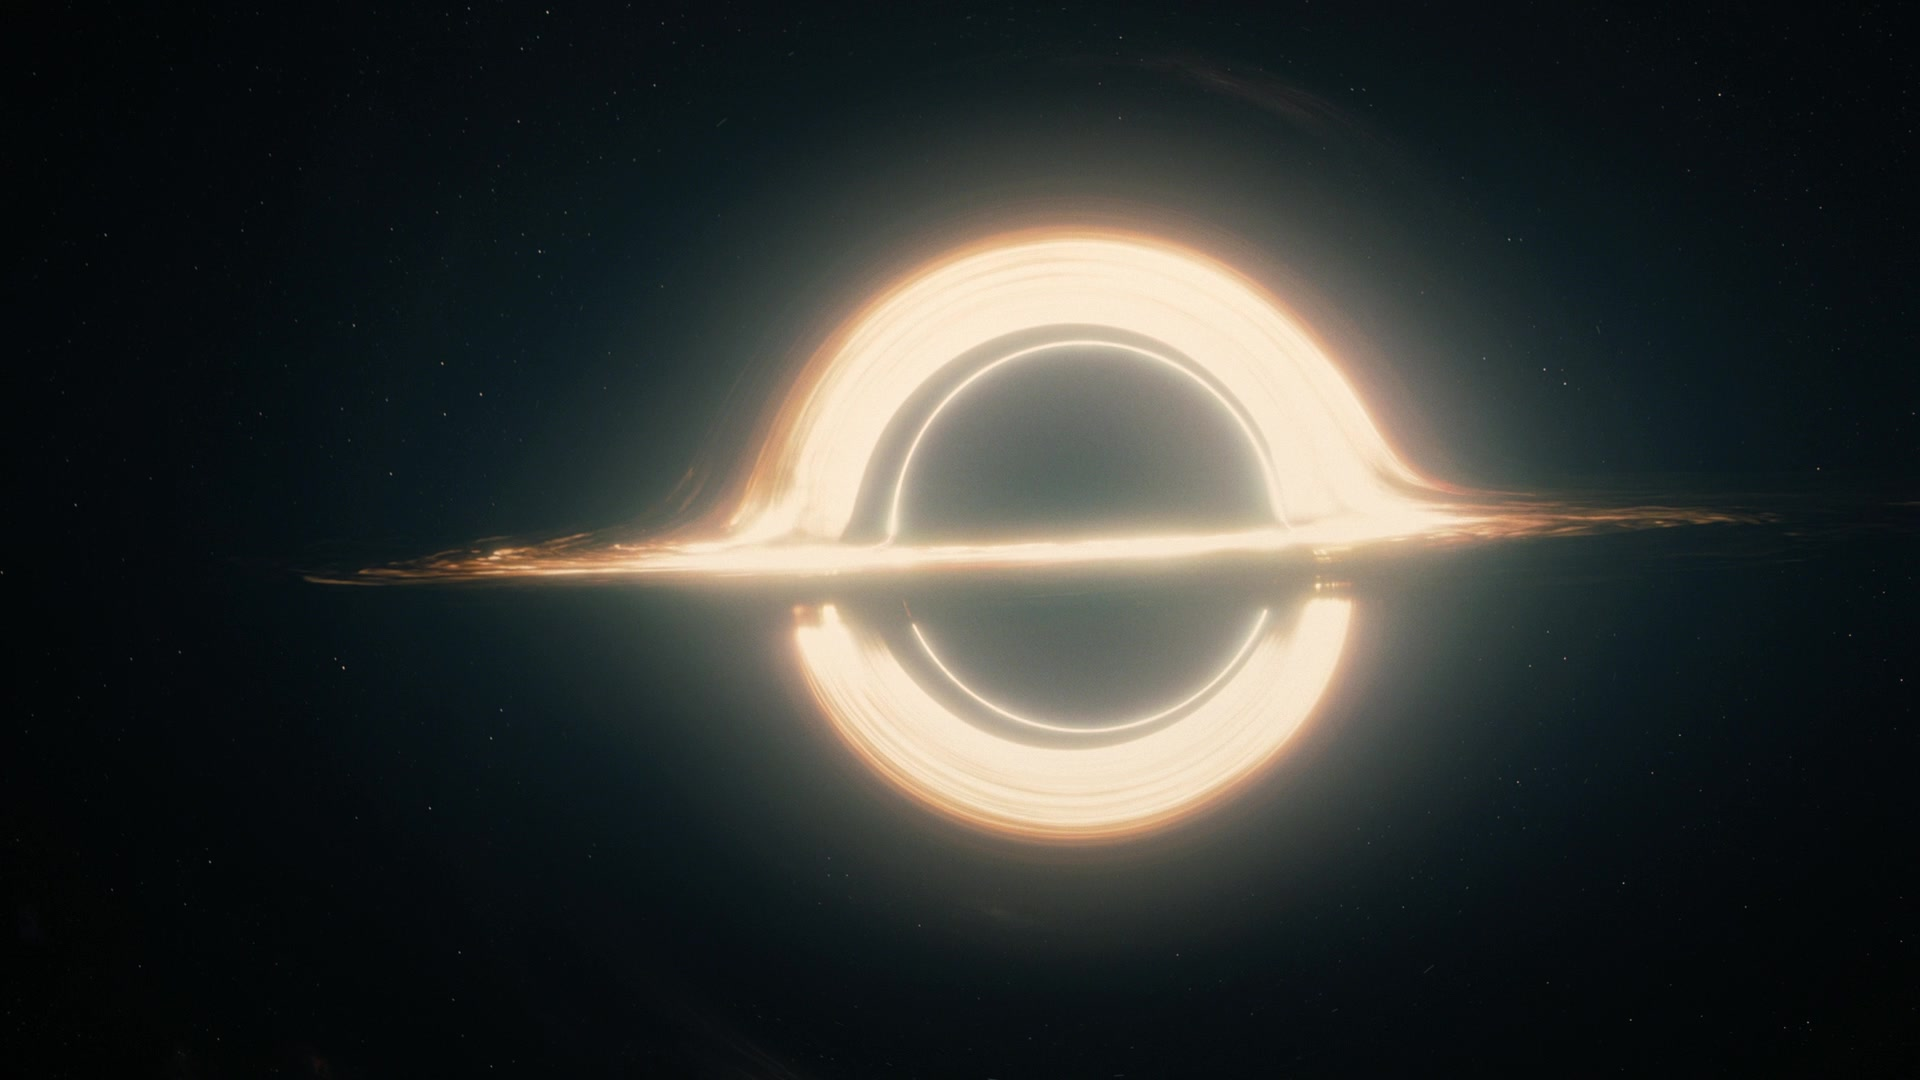
\includegraphics[width=\textwidth]{images/1200899.jpg}
		\end{figure}
	\end{frame}
	\begin{frame}
		Spoiler alert!
	\end{frame}
	\begin{frame}{"...but they constructed this 3-dim. (dimensional) space inside their 5-dim. reality to allow you to understand it..."}
			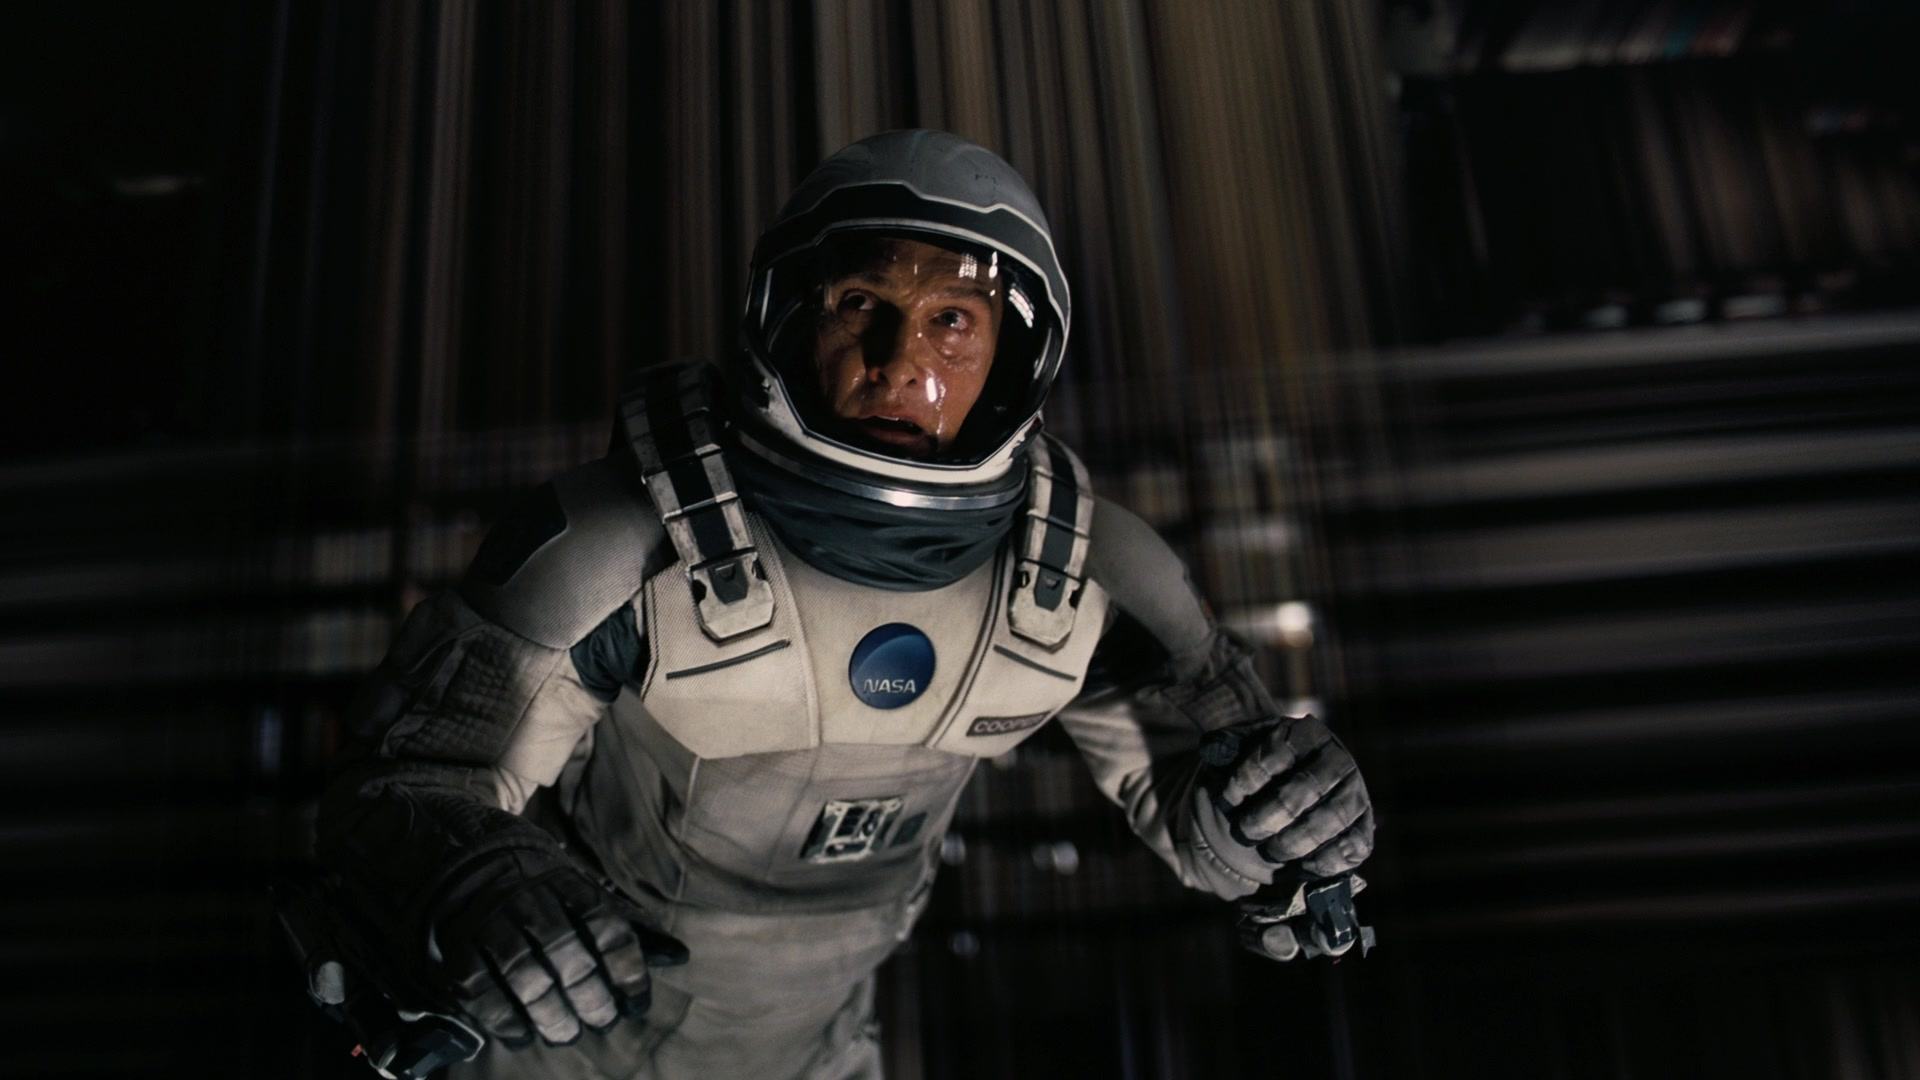
\includegraphics[width=\textwidth]{images/1201308.jpg}		
	\end{frame}
	\begin{frame}{Einstein's Theory of General Relativity}
		\begin{equation*}
			R_{ab} - \frac{1}{2} g_{ab} R = 8\pi G_N T_{ab}
		\end{equation*}
	\end{frame}
	\begin{frame}{Metric $g$}
		\begin{columns}
			\begin{column}{0.5\textwidth}
				Minkowski metric (flat)
					\begin{equation*}
						g = -dt^2 + dx^2 + dy^2 + dz^2
					\end{equation*}
			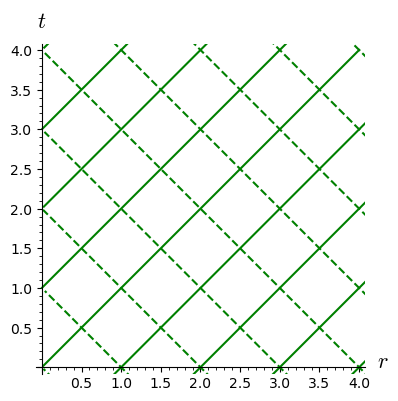
\includegraphics[width=0.4\textwidth]{images/conformal_Minkowskiindex.png}						
			\end{column}
			\begin{column}{0.5\textwidth}  %%<--- here
				Schwarzschild (static, non-spinning black hole) metric
					\scalebox{0.5}{%
						$g = -d\tau^2 = -\left( 1 - \frac{r_s}{r} \right) dt^2 + \left( 1 -\frac{r_s}{r} \right)^{-1} dr^2 + r^2 (d\theta^2 + \sin^2{\theta} d\phi^2)$
				}
			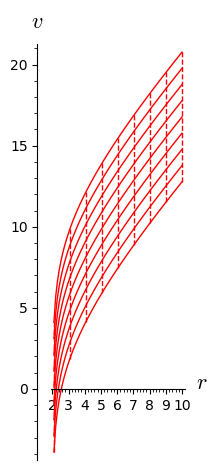
\includegraphics[width=0.4\textwidth]{images/SM_Schwarzschild_BoyerLindquistplotindex.png}						
			\end{column}
		\end{columns}
	\end{frame}
\end{document}